\chapter{Basic fluid simulation}

In order to implement the more advanced fluid simulation techniques, a proper basic fluid simulation is an essential starting point. For this project an Eulerian fluid method has been used, based on the techniques described in "Real-Time Fluid Dynamics For Games" by Jos Stam.

The techniques and tricks described in this paper are directly ported into the fluid simulation application used in this project. This is the case for basic physics, the grid structure used to calculate both the density and velocity fields as well as the basic solving routine for fluid simulations. The part describing the boundaries has been implemented and extended to work for the physical simulation bounding box as well as for fixed objects within the simulation.

The basic fluid simulation is also extended with mouse interaction. By clicking and dragging the mouse, a force can be added to the simulation.

\begin{figure}[htb!]
    \centering
    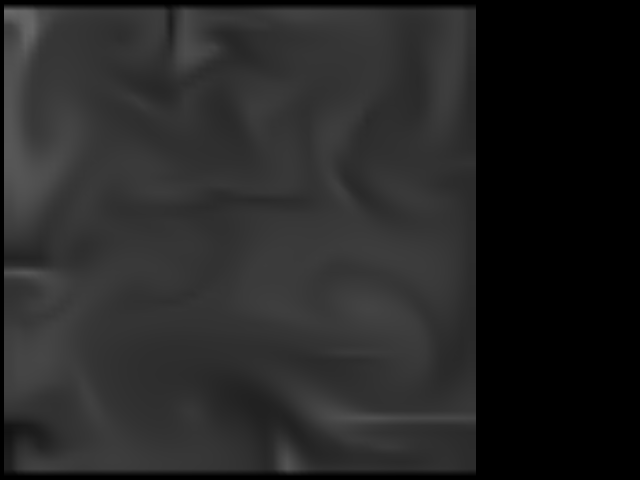
\includegraphics[width=0.6\textwidth]{images/BasicFluid}
    \caption{A scene of a fluid flowing through a bounded area.}
    \label{fig:Basic_fluid}
\end{figure}